\section{研究相关理论}
\subsection{排队论}
排队是在日常生活中经常遇到的现象,如顾客到商店购买物品、病人到医院看病常常
要排队。此时要求服务的人数超过服务机构的容量,即到达
的顾客不能立即得到服务,因而出现了排队现象。这种现象不仅在个人日常生活中出现,
电话局的占线问题,车站、码头等交通枢纽的车船堵塞和疏导,故障机器的停机待修,,水库
水量的存储调节等都是有形或无形的排队现象。由
于顾客到达和服务时间的随机性,可以说排队现象几乎是不可避免的。
如果增添服务设备,就要增加投资或发生空闲浪费;如果服务设备太少,排队现象就
会严重,对顾客个人和对社会都会带来不利影响。因此,管理人员必须考虑如何在这两者
之间取得平衡,经常检查目前处理是否得当,研究今后改进对策,以期提高服务质量,降低
成本\cite{ycx, jtgc}。

排队模型常表示成 $X/Y/Z/A/B/C$ (相继到达的间隔时间/服务时间的分布/服务台的数目/容量限制/客源数目/服务规则)形式,
对于一个公交站台可以表示成标准的 $M/M/1$ 模型,该系统的特点:

1.输入过程———顾客源是无限的,顾客单个到来,相互独立,一定时间的到达数服
从泊松分布,到达过程已是平稳的。

2.排队规则———单队,且对队长没有限制,先到先服务。

3.服务机构———单服务台,各顾客的服务时间是相互独立的,服从相同的负指数
分布。

此外,还假定到达间隔时间和服务时间是相互独立的。

已知 $M/M/1$ 模型到达规律服从参数为 $\lambda$ 的泊松分布,服务时间服从参数为 $\mu$ 的负指数分布,
给出 $t$ 时刻状态为 $n$ (系统中有 $n$ 个顾客)的概率 $P_{n}(t)$,系统的状态方程可以表示为:
\begin{equation}\label{fomula1}
    \begin{cases}
        -\lambda P_0 + \mu P_1 = 0
        \\
       \lambda p_{n - 1} + \mu P_{n + 1} - (\lambda + \mu)P_n = 0 \qquad n\ge 1
       \end{cases}
\end{equation}

式~\ref{fomula1}~是关于 $P_{n}$ 的差分方程,它表明的各状态之间的转移关系如图~\ref{fig21}~所示。

\begin{figure}[h]
\centering
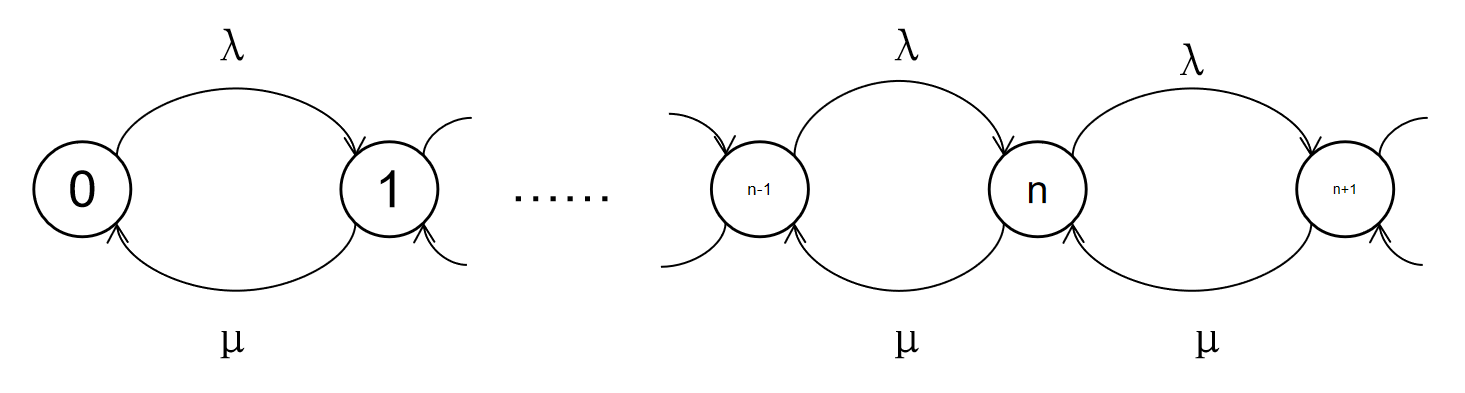
\includegraphics[width=0.80\textwidth]{figs/chap02/fig21.png}
\caption{M/M/1模型状态转移示意图}
\label{fig21}
\end{figure}


解决排队问题首先要根据原始资料作出顾客到达间隔和服务时间的经验分布,然后
按照统计学的方法(例如 $\chi^2$ 检验法)以确定合于哪种理论分布,并估计它的参数值,常用的分布函数有泊松分布、负指数分布、爱尔郎分布。
\subsection{运输问题}
在经济建设中,经常碰到物资调运问题,在若干生产基地,根据已有的交通网,应如何制订调运方案,将这些物资运到各消费地点,
而总运费要最小。这问题可用以下数学语言描述。

已知有 $m$ 个生产地点 $A_i$ , $i = 1, 2, …, m$ 。可供应某种物资, 其供应量(产量)分别为
$a_i$ , $ i = 1, 2, …, m$ ,有 $n$ 个销地 $B_j$ , $ j = 1, 2,…, n$ ,其需要量分别为 $b_j$ , $ j = 1, 2, …, n$ ,从 $A_i$ 到
$B_j$ 运输单位物资的运价(单价)为 $c_{ij}$。

若从 $x_{ij}$ 表示从 $A_i$ 到 $B_j$ 的运量,在产销平衡的条件下,要求总运费最小的调用方案,
可求解以下数学模型:
\begin{equation}\label{fomula2}
    \begin{array}{l} 
        \min z=\sum_{i=1}^{m} \sum_{j=1}^{n} a_{i j} x_{i j} \\
        \left\{\begin{array}{l}
        \sum_{i=1}^{m} x_{i j}=b_{j}, \quad j=1,2, \cdots, n \\
        \sum_{j=1}^{n} x_{i j}=a_{i}, \quad i=1,2, \cdots, m \\
        x_{i j} \geqslant 0
        \end{array}\right.
        \end{array}
\end{equation}

式~\ref{fomula2}~包含 $m \times n$ 个变量, $m+n$ 个约束方程对产销平衡的运输问题,由于有以下关系式存在:
$$\sum_{j=1}^{n} b_j = \sum_{i = 1}^{m} \left ( \sum_{j=1}^{n} \right ) = \sum_{j=1}^{n} \left ( \sum_{i=1}^{m} \right ) = \sum_{i=1}^{m} a_i$$

模型最多只有 $m+n-1$ 个独立约束方程。由于以上特征,所以求解运输问题时,
可用比较简便的计算方法,习惯上称为表上作业法。

\subsection{线性规划}
在生产管理和经营活动中经常提出一类问题, 即如何合理地利用有限资源,以便得到最好的经济效果,线性规划由此产生。
线性规划问题有各种不同的形式,将多种形式的数学模型统一变换为标准型式。规定的标准型式为:
$$\begin{aligned}
    & \max z =\sum_{j=1}^{n} c_{j} x_{j} \\
    & \left\{\begin{array}{l}
    \sum_{j=1}^{n} a_{i j} x_{j}=b_{i}, \quad i=1,2, \cdots, m \\
    x_{j} \geqslant 0, \quad j=1,2, \cdots, n
    \end{array}\right.
    \end{aligned}$$

    在实际数值计算中,更常用的是线性规划的矩阵形式:
$$
\begin{aligned}
    &max z=CX \\
    &AX = b\\
    &X \ge 0
\end{aligned}
$$

其中:
$$
\begin{pmatrix}
    a_{11}  & a_{12} &… &a_{1n} \\
     … &  …& &…\\
     a_{m1} & a_{m2} &…&a_{mn}
    \end{pmatrix}=\left ( P_1,P_2,…,P_n \right ) 
    ;0=\begin{bmatrix}
     0\\
     0\\
     …\\
    0
\end{bmatrix}
$$



A——约束条件的 $x \times n$ 维系数矩阵,一般 $m < n$;

b——资源向量;

C——价值向量

X——决策变量向量。


\subsection{动态规划}
在生产和科学实验中,有一类活动的过程,由于它的特殊性,可将过程分为若干个互
相联系的阶段,在它的每一个阶段都需要作出决策,从而使整个过程达到最好的活动效
果。因此,各个阶段决策的选取不是任意确定的,它依赖于当前面临的状态,又影响以后
的发展。当各个阶段决策确定后,就组成了一个决策序列,因而也就决定了整个过程的一
条活动路线。这种把一个问题可看作是一个前后关联具有链状结构的多阶段过程(如
图~\ref{fig22}~所示)就称为多阶段决策过程,也称序贯决策过程。这种问题就称为多阶段决策
过程。
\begin{figure}[h]
    \centering
    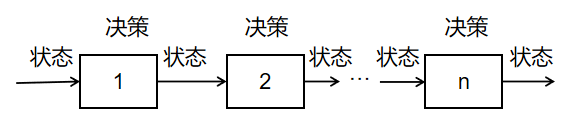
\includegraphics[width=0.80\textwidth]{figs/chap02/dp.png}
    \caption{多阶段决策示意图}
    \label{fig22}
\end{figure}

在多阶段决策问题中,各个阶段采取的决策,一般来说是与时间有关的,决策依赖于
当前的状态,又随即引起状态的转移,一个决策序列就是在变化的状态中产生出来
的,故有“动态”的含义。因此,把处理它的方法称为动态规划方法。

\subsection{图与网络模型}
图论是应用十分广泛的运筹学分支,它已广泛地应用在物理学、化学、控制论、信息
论、科学管理、电子计算机等各个领域。在实际生活、生产和科学研究中,有很多问题可以
用图论的理论和方法来解决。例如,运输系统的设计,再例如,各种通信网
络的合理架设,交通网络的合理分布等问题,应用图论的方法求解都很简便\cite{gycx}。

\subsection{对策论}
对策论亦称竞赛论或博弈论,是研究具有斗争或竞争性质现象的数学理论和方法。
一般认为,它是现代数学的一个新分支,是运筹学的一个重要学科。对策论发展的历史并
不长,但由于它研究的问题与政治、经济、军事活动乃至一般的日常生活等有着密切联系,
并且处理问题的方法具有明显特色,所以日益引起广泛注意。
对策问题本质上都由三个要素组成:

1.局中人——在一个对策行为(或一局对策)中, 有权决定自己行动方案的对策参加者, 称为局中
人。通常用 $I$ 表示局中人的集合。

2.策略集——一局对策中,可供局中人选择的一个实际可行的完整的行动方案称为一个策略。参
加对策的每一局中人 $i$ , $i \in I$ 都有自己的策略集 $S_i$ 。

3.赢得函数——在一局对策中,各局中人选定的策略形成的策略组称为一个局势,即若 $S_i$ 是第 $i$ 个局中人的一个策略,则 $n$ 个局中人的策略组
$$
s = \left(s_1,s_2,…,s_n\right)
$$
就是一个局势。对任一局势 $s \in S$ ,局中人 $i$ 可以得到一个赢得函数 $H_i(s)$

\subsection{VSP问题}
车辆调度问题(vehicle scheduling problem, VSP)是由 Dantzig 和 Ramser 于 1959 年
提出的,虽经多人潜心研究,但由于其复杂性大,目前仍未找到多项式算法,现有研究多把精力集中于研究高质量的启发式算法方面。
启发式方法是寻求解决问题的一种方法和策略;它也可以是面向某种具体问题的一种求解方法。它建立在人们经验和判断的基础之上,
体现了人的主观能动作用和创造力。

VSP问题的常规形式一般指:对一系列发货点和收货点,组织适当的行车路线,使车
辆有序地通过它们,在满足一定的约束条件下(例如货物需求量与发送量、交发货时间、车
量容量限制、行驶里程限制、行驶时间限制等),力争实现一定的目标(如空驶里程最短,运
输费用极小,车辆按时到达,使用车辆数量尽可能少等)。车辆调度问题的分类法很多,
例如可根据车辆满载与否分为满载问题与非满载问题,
根据可用车场数分为单车场问题与多车场问题,根据可用车辆的车型数分为单车型问题
与多车型问题,根据决策者的要求分为单目标问题与多目标问题等。


\subsection{离散事件仿真框架SimPy}
SimPy是一个进程驱动的基于Python语言的离散事件仿真框架,
SimPy中的进程由Python生成器函数定义,例如:用于对客户、车辆或代理等活动组件进行建模,SimPy还提供各种类型的共享资源。
模拟可以实时执行按时序或通过手动逐步执行事件。
